
\documentclass[12pt,a4paper]{article}

\usepackage[utf8]{inputenc} %Türkçe karakterler için
\usepackage[T1]{fontenc}
\usepackage{listings}

\usepackage{pdfpages}
\usepackage{geometry}
\usepackage{graphicx}
\usepackage{times}
\usepackage{graphicx}
\usepackage[nottoc]{tocbibind}
\usepackage{url}

\usepackage{color}
 
\definecolor{codegreen}{rgb}{0,0.6,0}
\definecolor{codegray}{rgb}{0.5,0.5,0.5}
\definecolor{codepurple}{rgb}{0.58,0,0.82}
\definecolor{backcolour}{rgb}{0.95,0.95,0.92}
 
\lstdefinestyle{mystyle}{
	frame=single,
    commentstyle=\color{codegreen},
    keywordstyle=\color{magenta},
    numberstyle=\tiny\color{codegray},
    stringstyle=\color{codepurple},
    basicstyle=\footnotesize,
    breakatwhitespace=false,         
    breaklines=true,                 
    captionpos=b,                    
    keepspaces=true,                 
    numbers=left,                    
    numbersep=5pt,                  
    showspaces=false,                
    showstringspaces=false,
    showtabs=false,                  
    tabsize=3
}
 
\lstset{style=mystyle}

\begin{document}

    \pagenumbering{gobble}
    \renewcommand{\abstractname}{Abstract}
\begin{titlepage}
    \begin{center}
        \begin{large}
            \vspace*{0.5cm}
            GAZİ UNIVERSITY \\
            ENGINEERING FACULTY \\
            COMPUTER ENGINEERING

            \vfill
            BM479E PARALLEL COMPUTER ARCHITECTURES \\
            AND 
            PROGRAMMING

            \vfill
            Estimating the Value of PI by Monte Carlo Method \\
            Using Message Passing Interface in C Programming Language

            \vfill
            \begin{abstract}
            In this assignment, value of pi has been calculated using
            Monte Carlo method. MPI has been used for parallelizing the code.
            A little benchmarking has also been presented for performance measurement issues.
            \end{abstract}
        
            \vfill
            141180001\\Abdullah Akalın\\abdullah.akalin@gazi.edu.tr

            \vfill
            \vspace{0.5cm}
            31.10.2017
        \end{large}
    \end{center}
\end{titlepage}

    \newpage

    \pagenumbering{roman}
    \tableofcontents
    \newpage

    \pagenumbering{arabic}

    \section{Introduction}
    Monte Carlo method states that, given a square located at the origin --assuming lower left corner is placed at (0,0) coordinates-- which has an
    arc in it (one-forth of a whole circle) as in the \figurename{} \ref{fig:sq}, the proportion of dots inside the arc to total dots randomly put in this square area is equal to pi/4. \cite{llnl}

    \begin{figure}[!h]
        \begin{center}
            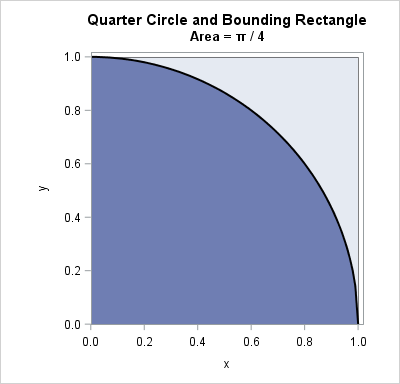
\includegraphics[width=200px]{resimler/arc.png}
            \caption{A unit square placed at the origin. \cite{arc}}
            \label{fig:sq}
        \end{center}
    \end{figure}

    \subsection{Parallelization}
    In this problem, putting randomly generated dots inside the square area is an independent job. Hence, it can be done simultaneously
    by any number of processors. After putting all the dots defined by the user, the value of pi can be readily estimated.

    \section{Application}
    \subsection{Program}
        In this program, I have used C as programming language and MPI for parallelization.
        The program begins with necessary pre-processor commands as listed below:
        \begin{lstlisting}
        #include <stdio.h>
        #include <stdlib.h>
        #include <mpi.h>
        #include <time.h>
        #include <math.h>
        \end{lstlisting}

        After that, in the \texttt{main} function, I have defined necessary variables.
        \begin{itemize}
            \item pid: Holds the current processor number.
            \item nop: Holds the total number of processors.
            \item TOTAL\_NUMBER\_OF\_POINTS: Holds the total number of dots that will be plotted in the square area.
            \item inside\_points: Holds points that are placed inside the arc.
            \item current\_total: Holds the number of points placed so far.
            \item gl\_inside\_points and gl\_current\_total: Hold cumulative values of the upper ones without "gl" prefix.
            \item pi: Holds estimated pi value.
            \item time\_measurement: Holds the elapsed time.
        \end{itemize}
        \begin{lstlisting}
        int pid;
        int nop;
        const int TOTAL_NUMBER_OF_POINTS = atoi(argv[1]);
        int inside_points = 0;
        int current_total = 0;
        int gl_inside_points;
        int gl_current_total;
        double pi;
        double time_measurement;
        \end{lstlisting}

        Below, MPI initialization procedures are being done and necessary information is being gathered such as rank and size.
        Also a barrier has been set for synchronizing in time measurement.
        \begin{lstlisting}
        MPI_Init(&argc, &argv);
        MPI_Barrier(MPI_COMM_WORLD);
        time_measurement = - MPI_Wtime();
        MPI_Comm_rank(MPI_COMM_WORLD, &pid);
        MPI_Comm_size(MPI_COMM_WORLD, &nop);
        \end{lstlisting}

        The parallel part of the program. After seeding the rand function, every processor runs their own portion of the loop and puts dots.
        If the magnitude of the vector (x,y) is less than 1, then the dot is inside the arc. In this case the inside point counter is incremented.
        \begin{lstlisting}
        srand(pid);
     
        for(int i = pid; i < TOTAL_NUMBER_OF_POINTS; i += nop)
        {
           double random_x = (double)rand() / (double)RAND_MAX;
           double random_y = (double)rand() / (double)RAND_MAX;
           double magnitude = random_x * random_x + random_y * random_y;
     
           if(magnitude <= 1)
              inside_points++;
           current_total++;
        }
        \end{lstlisting}

        Each processor adds its own number of dots to the global variables which will be
        readible for processor 0.
        Also, it is now okey to calculate the estimated time and finalize MPI.
        \begin{lstlisting}
        MPI_Reduce(&inside_points, &gl_inside_points,
            1, MPI_INT, MPI_SUM, 0, MPI_COMM_WORLD);
        MPI_Reduce(&current_total, &gl_current_total,
            1, MPI_INT, MPI_SUM, 0, MPI_COMM_WORLD);

        time_measurement += MPI_Wtime();
        MPI_Finalize();
        \end{lstlisting}

        If no more dots are being waited, then calculate pi and print necessary information to \texttt{stdout}.
        \begin{lstlisting}
        if(gl_current_total == TOTAL_NUMBER_OF_POINTS)
        {
           pi = 4 * (double)gl_inside_points / (double)gl_current_total;
           printf("%d,%d,%f,%f\n", nop, TOTAL_NUMBER_OF_POINTS, time_measurement, pi);
        }
        \end{lstlisting}
    
    \subsection{Scripts}
    These scripts are written for analyzing the performance of the program. The outputs are simply forwarded to csv files
    to plot the graphs.

    This script runs the program 100000000 times starting with 1 dot to 1.000.000.000 dots, using 4 processors.
    \lstinputlisting{../analysis/point.sh}

    This script runs the program 8 times starting with 1 processor to 8 processors, 1.000.000.000 dots for each.
    \lstinputlisting{../analysis/time.sh}

    \section{Analysis and Benchmarking}
    The program has been run at full capacity. Can be seen in \figurename{} \ref{cpu}.
    \begin{figure}[!h]
        \begin{center}
            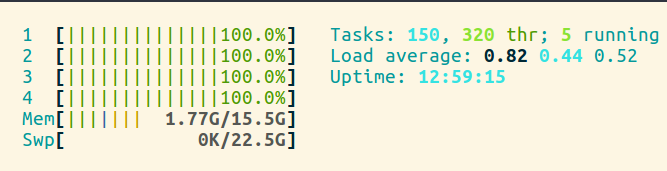
\includegraphics[width=\linewidth]{resimler/cpus.png}
            \caption{CPU usage.}
            \label{cpu}
        \end{center}
    \end{figure}

    Output of processes can be seen in \figurename{} \ref{ps}.
    \begin{figure}[!h]
        \begin{center}
            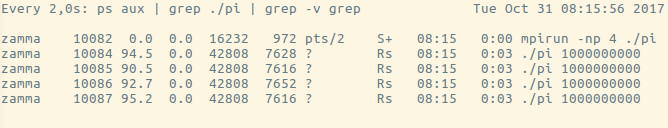
\includegraphics[width=\linewidth]{resimler/ps.png}
            \caption{Running 4 instances.}
            \label{ps}
        \end{center}
    \end{figure}

    Estimation of pi by number of points is shown in \figurename{} \ref{pnt}.
    \begin{figure}[!h]
        \begin{center}
            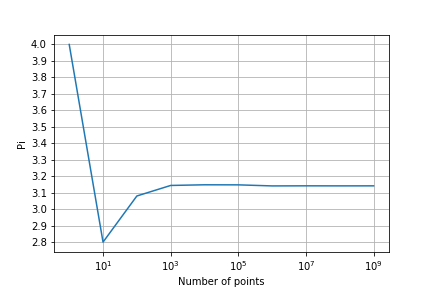
\includegraphics[width=200px]{resimler/point.png}
            \caption{Pi convergence with respect to number of dots placed.}
            \label{pnt}
        \end{center}
    \end{figure}

    Performance measurement can be seen in \figurename{} \ref{perf}.
    \begin{figure}[!h]
        \begin{center}
            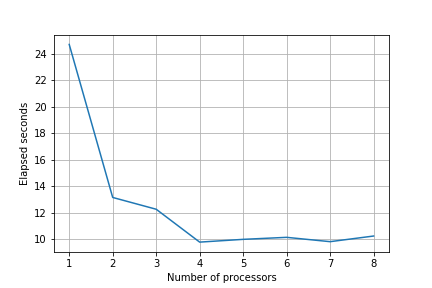
\includegraphics[width=200px]{resimler/proc.png}
            \caption{Performance measurement by time.}
            \label{perf}
        \end{center}
    \end{figure}

    \newpage
    \appendix
    \section{Source Code}
    \lstinputlisting{../pi.c}

    \newpage
    \section{Scripts}
    \lstinputlisting{../analysis/point.sh}
    \lstinputlisting{../analysis/time.sh}

    \newpage
    \section{Script Outputs}
    \lstinputlisting{../analysis/point_data.csv}
    \lstinputlisting{../analysis/processor_data.csv}

    \newpage
    \bibliography{kaynakca/kaynakca}
    \bibliographystyle{ieeetr}

\end{document}


